%%%%%%%%%%%%%%%%%%%%%%%%%%%%%%%%%%%%%%%%%
% Programming/Coding Assignment
% LaTeX Template
%
% This template has been downloaded from:
% http://www.latextemplates.com
%
% Original author:
% Ted Pavlic (http://www.tedpavlic.com)
%
% Note:
% The \lipsum[#] commands throughout this template generate dummy text
% to fill the template out. These commands should all be removed when 
% writing assignment content.
%
% This template uses a Perl script as an example snippet of code, most other
% languages are also usable. Configure them in the "CODE INCLUSION 
% CONFIGURATION" section.
%
%%%%%%%%%%%%%%%%%%%%%%%%%%%%%%%%%%%%%%%%%

%----------------------------------------------------------------------------------------
%	PACKAGES AND OTHER DOCUMENT CONFIGURATIONS
%----------------------------------------------------------------------------------------

\documentclass{article}
\usepackage[english]{babel}
\usepackage{amsmath}
\usepackage{fancyhdr} % Required for custom headers
\usepackage{lastpage} % Required to determine the last page for the footer
\usepackage{extramarks} % Required for headers and footers
\usepackage[usenames,dvipsnames]{color} % Required for custom colors
\usepackage{graphicx} % Required to insert images
\usepackage{subcaption}
\usepackage{listings} % Required for insertion of code
\usepackage{courier} % Required for the courier font
\usepackage{lipsum} % Used for inserting dummy 'Lorem ipsum' text into the template
\usepackage{dirtytalk}
% Margins
\topmargin=-0.45in
\evensidemargin=0in
\oddsidemargin=0in
\textwidth=6.5in
\textheight=9.0in
\headsep=0.25in

\linespread{1.1} % Line spacing

% Set up the header and footer
\pagestyle{fancy}
\lhead{\hmwkAuthorName} % Top left header
\chead{\hmwkClass\ (\hmwkClassTime): \hmwkTitle} % Top center head
%\rhead{\firstxmark} % Top right header
\lfoot{\lastxmark} % Bottom left footer
\cfoot{} % Bottom center footer
\rfoot{Page\ \thepage\ of\ \protect\pageref{LastPage}} % Bottom right footer
\renewcommand\headrulewidth{0.4pt} % Size of the header rule
\renewcommand\footrulewidth{0.4pt} % Size of the footer rule

\setlength\parindent{0pt} % Removes all indentation from paragraphs

%----------------------------------------------------------------------------------------
%	CODE INCLUSION CONFIGURATION
%----------------------------------------------------------------------------------------

\definecolor{MyDarkGreen}{rgb}{0.0,0.4,0.0} % This is the color used for comments
\lstloadlanguages{Perl} % Load Perl syntax for listings, for a list of other languages supported see: ftp://ftp.tex.ac.uk/tex-archive/macros/latex/contrib/listings/listings.pdf
\lstset{language=Perl, % Use Perl in this example
        frame=single, % Single frame around code
        basicstyle=\small\ttfamily, % Use small true type font
        keywordstyle=[1]\color{Blue}\bf, % Perl functions bold and blue
        keywordstyle=[2]\color{Purple}, % Perl function arguments purple
        keywordstyle=[3]\color{Blue}\underbar, % Custom functions underlined and blue
        identifierstyle=, % Nothing special about identifiers                                         
        commentstyle=\usefont{T1}{pcr}{m}{sl}\color{MyDarkGreen}\small, % Comments small dark green courier font
        stringstyle=\color{Purple}, % Strings are purple
        showstringspaces=false, % Don't put marks in string spaces
        tabsize=5, % 5 spaces per tab
        %
        % Put standard Perl functions not included in the default language here
        morekeywords={rand},
        %
        % Put Perl function parameters here
        morekeywords=[2]{on, off, interp},
        %
        % Put user defined functions here
        morekeywords=[3]{test},
       	%
        morecomment=[l][\color{Blue}]{...}, % Line continuation (...) like blue comment
        numbers=left, % Line numbers on left
        firstnumber=1, % Line numbers start with line 1
        numberstyle=\tiny\color{Blue}, % Line numbers are blue and small
        stepnumber=5 % Line numbers go in steps of 5
}

% Creates a new command to include a perl script, the first parameter is the filename of the script (without .pl), the second parameter is the caption
\newcommand{\perlscript}[2]{
\begin{itemize}
\item[]\lstinputlisting[caption=#2,label=#1]{#1.pl}
\end{itemize}
}

%----------------------------------------------------------------------------------------
%	DOCUMENT STRUCTURE COMMANDS
%	Skip this unless you know what you're doing
%----------------------------------------------------------------------------------------

% Header and footer for when a page split occurs within a problem environment
\newcommand{\enterProblemHeader}[1]{
%\nobreak\extramarks{#1}{#1 continued on next page\ldots}\nobreak
%\nobreak\extramarks{#1 (continued)}{#1 continued on next page\ldots}\nobreak
}

% Header and footer for when a page split occurs between problem environments
\newcommand{\exitProblemHeader}[1]{
%\nobreak\extramarks{#1 (continued)}{#1 continued on next page\ldots}\nobreak
%\nobreak\extramarks{#1}{}\nobreak
}

\setcounter{secnumdepth}{0} % Removes default section numbers
\newcounter{homeworkProblemCounter} % Creates a counter to keep track of the number of problems
\setcounter{homeworkProblemCounter}{0}

\newcommand{\homeworkProblemName}{}
\newenvironment{homeworkProblem}[1][Part \arabic{homeworkProblemCounter}]{ % Makes a new environment called homeworkProblem which takes 1 argument (custom name) but the default is "Problem #"
\stepcounter{homeworkProblemCounter} % Increase counter for number of problems
\renewcommand{\homeworkProblemName}{#1} % Assign \homeworkProblemName the name of the problem
\section{\homeworkProblemName} % Make a section in the document with the custom problem count
\enterProblemHeader{\homeworkProblemName} % Header and footer within the environment
}{
\exitProblemHeader{\homeworkProblemName} % Header and footer after the environment
}

\newcommand{\problemAnswer}[1]{ % Defines the problem answer command with the content as the only argument
\noindent\framebox[\columnwidth][c]{\begin{minipage}{0.98\columnwidth}#1\end{minipage}} % Makes the box around the problem answer and puts the content inside
}

\newcommand{\homeworkSectionName}{}
\newenvironment{homeworkSection}[1]{ % New environment for sections within homework problems, takes 1 argument - the name of the section
\renewcommand{\homeworkSectionName}{#1} % Assign \homeworkSectionName to the name of the section from the environment argument
\subsection{\homeworkSectionName} % Make a subsection with the custom name of the subsection
\enterProblemHeader{\homeworkProblemName\ [\homeworkSectionName]} % Header and footer within the environment
}{
\enterProblemHeader{\homeworkProblemName} % Header and footer after the environment
}

%----------------------------------------------------------------------------------------
%	NAME AND CLASS SECTION
%----------------------------------------------------------------------------------------

\newcommand{\hmwkTitle}{Assignment 3} % Assignment title
\newcommand{\hmwkDueDate}{Tuesday, March 19, 2017, 11pm} % Due date
\newcommand{\hmwkClass}{CSC411} % Course/class
\newcommand{\hmwkClassTime}{L0101} % Class/lecture time
\newcommand{\hmwkAuthorName}{Minh Nguyen (1000468059)} % Your name

%----------------------------------------------------------------------------------------
%	TITLE PAGE
%----------------------------------------------------------------------------------------

\title{
\vspace{2in}
\textmd{\textbf{\hmwkClass:\ \hmwkTitle}}\\
\normalsize\vspace{0.1in}\small{Due\ on\ \hmwkDueDate}\\
\vspace{0.1in}
\vspace{3in}
}

\author{\textbf{\hmwkAuthorName}}
%\date{} % Insert date here if you want it to appear below your name

%----------------------------------------------------------------------------------------

\begin{document}
\maketitle
\clearpage

\textbf{Instruction for reproducing the results:}
\begin{itemize}
\item \textit{naivebayes.py}: codes for part 1,2,3 as well as picking the samples from the data set.
\item \textit{logistic.py}: codes for part 4. 
\item \textit{compare\_nb\_log.py}: codes for part 6.
\item \textit{word2vec.py}: codes for part 7, 8.
\end{itemize}
The main program for each part is in a seperated function \textit{def part[i]()} where \textit{[i]} is the part of the assignment. For example, if you want to run part 8, you should go to file \textit{word2vec.py} and uncomment the line \textit{part8()}, then run the program to see the result. \\

Please download and extract \textit{review\_polarity.tar.gz} into the same folder that you save my codes. This is the raw movie review data set given by the professor.\\ 

As part of the submission, I also submitted \textit{report.zip} which consists all of the images used in the report. \\

%----------------------------------------------------------------------------------------
%	PART 1
%----------------------------------------------------------------------------------------
\clearpage
% To have just one problem per page, simply put a \clearpage after each problem
\begin{homeworkProblem}
\textbf{Dataset descriptions:} \\
The size of the training, validation and test datasets are 800, 200 and 200 respectively. Each set has an equal number of positive and negative reviews. Below is the summary of the number of unique words in each of dataset.
\begin{enumerate}
\item Training set: 800 images, 400 postive and 400 negative reviews.
\begin{itemize}
\item Number of unique words in positive reviews: 23303
\item Number of unique words in negative reviews: 21594
\item Total number of unique words: 32689
\end{itemize}
\item Test set: 200 images, 100 postive and 100 negative reviews.
\begin{itemize}
\item Number of unique words in positive reviews: 10200
\item Number of unique words in negative reviews: 9656
\item Total number of unique words: 15129
\end{itemize}
\item Validation set: 200 images, 100 postive and 100 negative reviews.
\begin{itemize}
\item Number of unique words in positive reviews: 10855
\item Number of unique words in negative reviews: 9728
\item Total number of unique words: 15687
\end{itemize}
\end{enumerate}

\textbf{Example of three key words} \\
We will look at how often the three words \say{Nice}, \say{Bad} and \say{Boring} occur in the training set. \\
\textbf{\say{enjoyed}}
\begin{itemize}
\item Number of occurences of \say{enjoyed} in the positive reviews: 26
\item Number of occurences of \say{enjoyed} in the negative reviews: 14
\end{itemize}

\textbf{\say{bad}}
\begin{itemize}
\item Number of occurences of \say{bad} in the positive reviews: 104
\item Number of occurences of \say{bad} in the negative reviews: 207
\end{itemize}

\textbf{\say{boring}}
\begin{itemize}
\item Number of occurences of \say{boring} in the positive reviews: 19
\item Number of occurences of \say{boring} in the negative reviews: 66
\end{itemize}

It can be seen from the result that the positive word \say{enjoyed} occurs almost twice times as often in the positive reviews than in negative reviews. In contrast, the negative words such as \say{boring} and \say{bad} occur more frequent in negative reviews than in positive reviews. This is because when people writing positive reviews are more likely to use good words like \say{enjoyed}, \say{happy}, \say{fun} to desribe their positive experience with the movie. Similarly, reviewers who had bad experience with the movie are more likely to use the words like \say{bad} and \say{boring} in their reviews. Therefore, it is totally feasible to make a prediction whether the review is positive or negative using just some keywords within the review. \\ 

\end{homeworkProblem}


%----------------------------------------------------------------------------------------
%	PART 2
%----------------------------------------------------------------------------------------
\clearpage
\begin{homeworkProblem}
\textbf{Tuning parameter m, k:} \\
I ran the Bayesian classifier on the validation set and observe the performance. I started with small values $m=1$ and $k=1$, the performance of the classier was less than 20 \% for both negative reviews and positive reviews. This was because multiple terms $P(a_i|class)$ were too small that when adding their logs $log(P(a_1|class)) + log(P(a_2 | class)) + ... + log(P(a_n|class) + log(0.5))$, the result was a big negative number, so $e^{log(P(a_1|class)) + log(P(a_2 | class)) + ... + log(P(a_n|class) + log(0.5))} = e^{-\infty} \approx 0$.  Because the number was so small that it could not be represented by the system, the OS rounded the number down to 0, this is called arithmetic underflow. Therefore the posterior $P(positive reviews |a_1, a_2, ..., a_n) = P(negative reviews |a_1, a_2, ..., a_n) = 0$ made it impossible to do the classification.\\

To fix the issue, I needed to scale up each of the term $P(a_i|class)$. We have that $P(a_i = 1|class) = \dfrac{count(a_i, class) + mk}{count(class) + k}$, the term k appears in both denominator and numerator but m only shows up in the numerator, so increasing m would only increase the numerator. I kept k constant at 1, and increased m by 50 at a time. As m increased, each term $P(a_i|class)$ is scaled up made it less likely that underflow could happen, increasing the performance of the classifier. When $m \approx 500.0$, the performance on the positive reviews of the validation set was 95\%, and the performance on the negative reviews was only 41 \%. Any m greater than 500 would make the scaled values to be too big, that is would cause arithmetic overflow. So I stopped increasing m at 500, and started adjusting k. \\

As k increased, the performance on the negative reviews improved slightly to 51 \% from 43 \%. However it would also made the performance on the positive reviews decrease to below 90 \%. From this point on ward, I just adjusted k and m by small amount until I had the highest average performance between the positive and negative reviews. Below are the recorded performances on the validation, test and train set with $k=3$ and $m=460$.\\

\begin{lstlisting}[language=Python]
-------------------Validation set performance-----------------
Performance on positie reviews: 90.0
Performance on negative reviews: 49.0
Overall result: 69.5
-------------------Test set performance-----------------
Performance on positie reviews: 92.0
Performance on negative reviews: 53.0
Overall result: 72.5
-------------------Train set performance-----------------
Performance on positie reviews: 93.25
Performance on negative reviews: 65.5
Overall result: 79.375
\end{lstlisting} 

The low performance on the negative reviews is due to the fact that the negative reviews are usually shorter than the positive reviews. This performance can be improved by using a larger training set, the current performance is based on a training set of 800 samples with 32689 unique words.

\end{homeworkProblem}

%----------------------------------------------------------------------------------------
%	PART 3
%----------------------------------------------------------------------------------------
\clearpage
\begin{homeworkProblem}
\textbf{Top 10 words that indicate the review is negative:} \\
if, ?, why, boring, worst, bad, better, it's, script, plot. \\

\textbf{Top 10 words that indicate the review is positive:} \\
best, great, also, him, makes, world, while, both, life, young. \\

\textbf{Note} Professor confirmed on Piazza that there is no need to remove punctutation such as \say{?}. \\

\textbf{Explaination}
A word is a strong indicator of a positive review if the posterior probability $P(positive review | word)$ is high and $P(negative review | word)$ is low. On the other hand, if $P(positive review | word)$ is low and $P(negative review | word)$ is high, then the review with that word is more likely to be negative.\\

From Bayesian rule, we have that $P(class | word) = \dfrac{P(word|class) P(class)} {P(word)}$. So $P(positive review | word) \propto P(word | positive review)$, and  $P(negative review | word) \propto P(word | negative review)$ as $P(class) = 0.5$ is constant since we picked an equal number of samples from each class. \\

Then if $P(word | positive review) - P(word | negative review)$ is high, $P(positive review | word) - P(negative review | word)$ is also high. I used Bayesian algorithm to calculate  $P(word | positive review)$ and $P(word | negative review)$ for each word, then I calculated the difference $P(word | positive review) - P (word | negative review)$ . The top 10 words that have highest $P(word | positive review) - P (word | negative review) $ are words that occur frequently in positive reviews but rarely in negative reviews, therefore is a strong positive preview's indication. And the bottom 10 words that have least $P(word | positive review) - P (word | negative review) $ are strong indications of negative reviews. \\

\end{homeworkProblem}

%----------------------------------------------------------------------------------------
%	PART 4
%----------------------------------------------------------------------------------------
\clearpage
\begin{homeworkProblem}
To choose the right regularization perameter, I observe the performance on the validation set. I first ran the program with $\lambda = 0$, so the high weights would not be penalized at all. The performance on the training set quickly went to 100 \% after 30 iterations, whereas the after 300 interations the performance on the validation set was barely 80 \%. Below is the learning curve obtained by running the program with no regularization. \\

\begin{figure*}[!ht]
\begin{center}
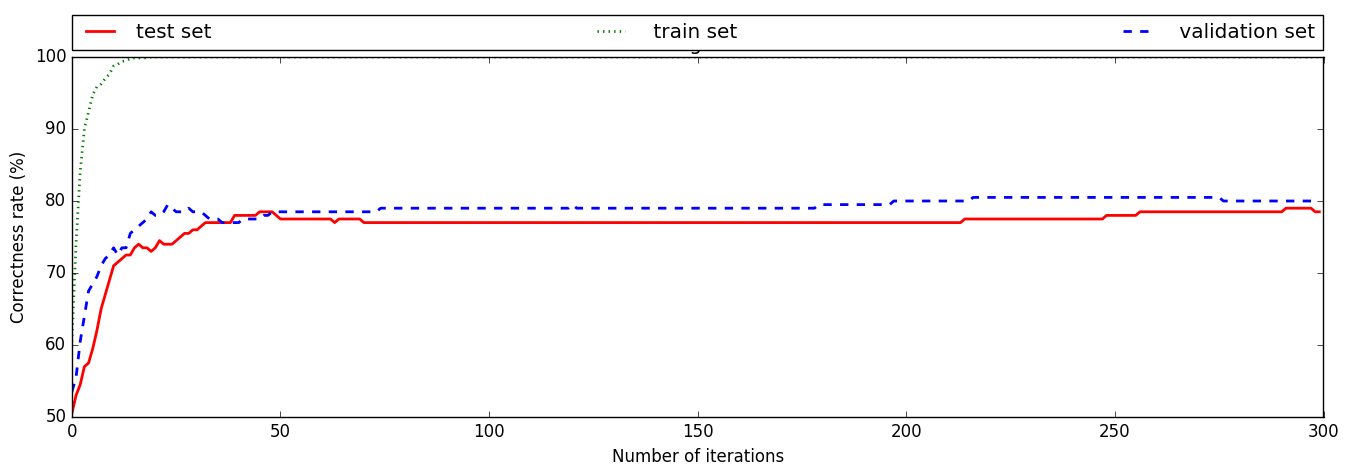
\includegraphics[width=.9\linewidth]{no_reg.png}
\caption{Learning curve with no regularization (i.e. $\lambda = 0$) based on 300 iterations.}
\end{center}
\end{figure*}

The large performance gap between training and test sets indicate that overfitting was occured. The model was better at learning the specific data in the training set than the general relationship. \\
To solve the issue, I started setting $\lambda$ to be some non-zero values. Iteratively, I tried to set $\lambda$ to be $0.1$, $1$, $10$, etc. and ploted the learning curves. I observed that as $\lambda$ got higher, the performance on the training set was decreasing while the performance on the validation set was increasing. This closed the performance gap, and therefore reduced the overfitting. At $\lambda=1000$, the performance on the validation and training sets were 84 \% and 94 \%, respectively. reduced the number of iterations to 200 from 300 because after 200 iterations, the performance on the validaton set was no longer improved. For any $\lambda > 1000$, the performances on all three sets decreased. So $\lambda = 1000$ was the best regulariaztion paraeter for my model. Below is the learning curve with the regularization applied.
\begin{figure*}[!ht]
\begin{center}
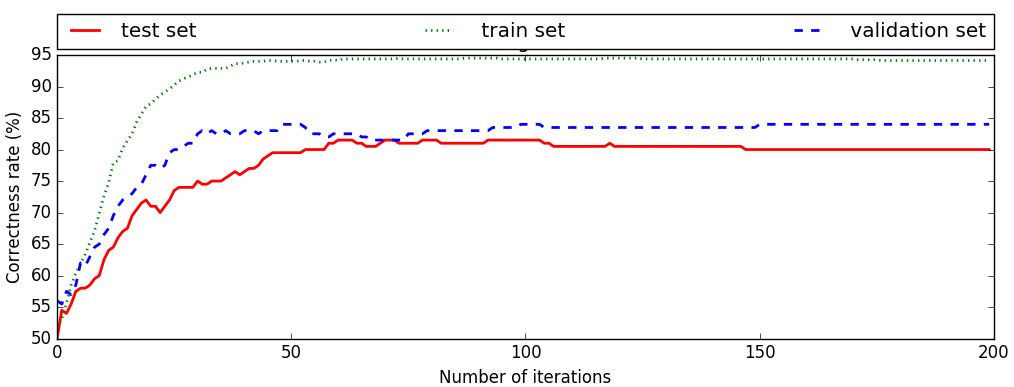
\includegraphics[width=.9\linewidth]{reg.png}
\caption{Learning curve with weight decay $(\lambda=1000$) based on 200 iterations. Note that the maximum value on the y axis is 95, not 100 like in the previou plot.}
\end{center}
\end{figure*}
\end{homeworkProblem}


%----------------------------------------------------------------------------------------
%	PART 5
%----------------------------------------------------------------------------------------
\clearpage
\begin{homeworkProblem}
\begin{equation}
\theta_0 + \theta_1 I_1 (x) + \theta_2 I_2 (x) + ... + \theta_k I_k (x) > \text{thr} \\
\end{equation}
\textbf{Naive Bayesian:}
Let k be the number of unique words in the training set, and x is the document.
\begin{equation}
\begin{split}
P(class_{positive} | a_1, ..., a_k) &= \dfrac{P(a_1, a_2, ..., a_k | class_{positive}) \times P (class_{positive})}{a_1, a_2, ..., a_k} \\
\implies P(class_{positive} | a_1, ..., a_k) &\propto P(a_1, a_2, ..., a_k | class_{positive}) \times P(class_{positive}) \\
\implies P(class_{positive} | a_1, ..., a_k) &\propto (P(a_1 | class_{positive}) \times ... \times P(a_k | class_{positive})) \times
 P(class_{positive}) \\
\implies P(class_{positive} | a_1, ..., a_k) &\propto log(P(a_1 | class_{positive})) + ... + log(P(a_k | class_{positive})) +
 log(P(class_{positive})) \\
\end{split} 
\end{equation} \\

Similarly, we get the following equation for the negative class.
\begin{equation}
\begin{split}
P(class_{negative} | a_1, ..., a_k) &\propto log(P(a_1 | class_{negative})) + ... + log(P(a_k | class_{negative})) +
 log(P(class_{negative})) \\
 \end{split}
\end{equation}

Let take the difference between the two.
\begin{equation}
\begin{split}
(2) - (3) &= (\sum_i^k(log(P(a_i|class_{positive})) - log(P(a_i|class_{negative})))) + (log(P(class_{positive})) - log(P(class _{negative})))
\end{split}
\end{equation}
If $(2) - (3) > 0$, it means that if \textbf{all} the unique words in the training set appear in the document, then it is more likely that the document is a positive review. Otherwise, if $(2) - (3) < 0$, there is higher chance that the document is a negative review. We can think of each term $(log(P(a_i|class_{positive})) - log(P(a_i|class_{negative}))$ in the summation as $\theta_i$. However, \textbf{not all} key words $a_i$ will be showed up in the test document. So we need an indicator function $I_i(x)$ that indicates if the key word $a_i$ is in the document x. If $a_i$ is in x, then $I_i(x) = 1$, otherwise $I_i(x) = 0$. Adding in the indicator function into the equation $(4)$, we have the following equation for doing classification:
\begin{equation}
\begin{split}
&= (\sum_i^k((log(P(a_i|class_{positive})) - log(P(a_i|class_{negative}))) I_i(x))) + (log(P(class_{positive})) - log(P(class _{negative}))) \\
&= (\sum_i^k(\theta_i \times I_i(x))) + (log(P(class_{positive})) - log(P(class _{negative}))) \\
&= (\sum_i^k(\theta_i \times I_i(x))) + \theta_0
\end{split}
\end{equation}

\textbf{Logistic Regression}
Assuming that we use one-hot encoding, we get two sets of weights, one for each of the two classes. This is similar to the two set of probabilities we got in Naive Bayesian algorithm. \\
$W_{positvereview} = \{W_{word1,+}, W_{word2,+}, ..., W_{wordk, +}\}$ \\
$W_{negativereview} = \{W_{word1,-}, W_{word2,-}, ..., W_{wordk, -}\}$ \\

We can define the classification functon as follow: \\
\begin{equation}
\begin{split}
&= ( \sum_i^k((W_{wordi, +} - W_{wordi, -}) I_i(x))) + (W_{bias+} - W_{bias-}) \\
&= ( \sum_i^k(\theta_i \times I_i(x)) ) + \theta_0 \\
\end{split}
\end{equation}
Similar to what we got with Bayesian classification, $I_i(x)$ i the indicator function that outputs 0 or 1 to indicate whether the key word i is in the document x. $\theta_i$ is $(W_{wordi, +} - W_{wordi, -})$ and $\theta_0$ is the weight bias.\\

\textbf{Note:} $+$ denotes the class positive review, and $-$ denotes the class negative review.
\end{homeworkProblem}


%----------------------------------------------------------------------------------------
%	PART 6
%----------------------------------------------------------------------------------------
\clearpage
\begin{homeworkProblem}
\textbf{Top 50 $\theta$ for positive reviews with Naive Bayesian classification:} 
\begin{lstlisting}[language=Python]
{'own': 0.030833333333333268, 'family': 0.02416666666666667, 'simple': 0.0266666
6666666684, 'years': 0.03750000000000009, 'see': 0.02416666666666667, 'human': 0
.03416666666666668, 'seen': 0.03166666666666673, 'subtle': 0.03249999999999997, 
'still': 0.026666666666666616, 'yet': 0.03499999999999992, 'best': 0.05416666666
6666696, 'perfect': 0.02499999999999991, 'different': 0.02416666666666667, 'thro
ughout': 0.026666666666666616, 'takes': 0.03166666666666651, 'true': 0.030833333
333333268, 'young': 0.03833333333333333, 'also': 0.054166666666666696, 'does': 0
.02416666666666667, 'between': 0.035833333333333384, 'performance': 0.0266666666
66666616, 'several': 0.03166666666666673, 'life': 0.06666666666666665, 'attentio
n': 0.02416666666666667, 'may': 0.03499999999999992, 'each': 0.03166666666666673
, 'most': 0.03749999999999987, 'job': 0.02416666666666667, 'others': 0.032499999
99999997, 'world': 0.05499999999999994, 'strong': 0.029166666666666563, 'friends
': 0.03166666666666673, 'him': 0.05083333333333351, 'begins': 0.0283333333333333
2, 'both': 0.043333333333333446, 'great': 0.044166666666666465, 'perfectly': 0.0
27499999999999858, 'especially': 0.033333333333333215, 'effective': 0.0258333333
33333375, 'always': 0.030833333333333268, 'brilliant': 0.030833333333333268, 'ma
ny': 0.03749999999999987, 'allows': 0.02416666666666667, 'will': 0.0283333333333
3332, 'while': 0.03916666666666657, 'performances': 0.03500000000000014, 'very':
 0.03333333333333344, 'american': 0.030000000000000027, 'makes': 0.0425000000000
00204, 'almost': 0.025000000000000133}
\end{lstlisting} 

\textbf{Top 50 $\theta$ for negative reviews with Naive Bayesian classification:} 
\begin{lstlisting}[language=Python]
{'just': -0.025833333333333153, 'give': -0.023333333333333206, "didn't": -0.0233
33333333333428, 'anyway': -0.022500000000000187, 'wasted': -0.026666666666666616
, 'awful': -0.025000000000000133, 'looks': -0.030833333333333268, 'if': -0.04750
00000000001, '!': -0.03249999999999997, 'plot': -0.03833333333333333, 'guess': -
0.026666666666666616, 'i': -0.02666666666666684, 'script': -0.04833333333333334,
 "it's": -0.040000000000000036, 'least': -0.03499999999999992, 'either': -0.0233
33333333333206, 'better': -0.03833333333333333, "wasn't": -0.025000000000000133,
 "there's": -0.02833333333333332, 'got': -0.023333333333333206, 'waste': -0.0250
00000000000133, 'decent': -0.022499999999999964, '?': -0.0691666666666666, 'supp
osed': -0.036666666666666625, 'poor': -0.02416666666666667, 'worse': -0.02416666
666666667, 'mess': -0.026666666666666616, 'material': -0.02499999999999991, 'rea
son': -0.02833333333333332, 'ridiculous': -0.02416666666666667, 'worst': -0.0549
9999999999994, 'nothing': -0.027499999999999858, 'why': -0.04083333333333328, 'l
ook': -0.025833333333333375, 'none': -0.027499999999999858, 'save': -0.022499999
999999964, 'talent': -0.022500000000000187, 'unfortunately': -0.0333333333333334
4, 'course': -0.022499999999999964, 'did': -0.02750000000000008, 'maybe': -0.033
333333333333215, 'lame': -0.02499999999999991, 'terrible': -0.023333333333333428
, 'thing': -0.029999999999999805, 'bad': -0.08583333333333343, 'stupid': -0.0341
6666666666668, "can't": -0.03166666666666673, 'boring': -0.039166666666666794, '
predictable': -0.02833333333333332, "isn't": -0.02833333333333332}
\end{lstlisting} 
\textbf{Top 50 $\theta$ for positive reviews with Logistic Regression classification:} 
\begin{lstlisting}[language=Python]
{'own': 0.013312923, 'simple': 0.012355411, 'years': 0.016862687, 'see': 0.01202
184, 'human': 0.015253512, 'subtle': 0.015125709, 'seen': 0.016072426, 'still': 
0.012846986, 'yet': 0.016108947, 'best': 0.025253143, 'perfect': 0.011767382, 't
hroughout': 0.012045614, 'takes': 0.013620302, 'true': 0.01362077, 'young': 0.01
529683, 'terrific': 0.011474546, 'also': 0.025604311, 'between': 0.015466765, 'p
erformance': 0.011917949, 'several': 0.014882077, 'life': 0.029041685, 'attentio
n': 0.011084631, 'may': 0.014872752, 'very': 0.016251992, 'each': 0.013253912, '
overall': 0.012112376, 'hilarious': 0.011038193, 'most': 0.016242225, 'job': 0.0
11477605, 'others': 0.015621452, 'world': 0.024853006, 'strong': 0.012559932, 'f
riends': 0.016162531, 'him': 0.023612441, 'begins': 0.012439251, 'both': 0.01898
8151, 'great': 0.020791847, 'perfectly': 0.013204739, 'especially': 0.016167773,
 'effective': 0.011887925, 'always': 0.013800211, 'brilliant': 0.015066012, 'per
formances': 0.015978094, 'allows': 0.012258044, 'will': 0.012324894, 'while': 0.
017829601, 'many': 0.015284918, 'american': 0.013127217, 'makes': 0.020303458, '
almost': 0.011035507}
\end{lstlisting} 
\textbf{Top 50 $\theta$ for negative reviews with Logistic Regression classification:} 
\begin{lstlisting}[language=Python]
{"isn't": -0.012588516, 'just': -0.01103092, 'give': -0.011644898, 'wasted': -0.
013344445, 'awful': -0.012129982, 'looks': -0.015486099, 'have': -0.010863103, '
if': -0.024498831, '!': -0.013051623, 'plot': -0.018612798, 'guess': -0.01262189
4, 'script': -0.024369545, "it's": -0.018512912, 'least': -0.016362293, 'better'
: -0.019479303, "wasn't": -0.012312988, "there's": -0.012758968, 'waste': -0.012
352165, '?': -0.032902829, 'either': -0.011666148, 'poor': -0.012486506, 'then':
 -0.010981265, 'worse': -0.01204066, 'mess': -0.013252348, 'material': -0.013801
686, 'director': -0.012016099, 'reason': -0.014537231, 'ridiculous': -0.01187721
5, 'worst': -0.027064471, 'nothing': -0.01420748, 'attempt': -0.011391882, 'why'
: -0.019721836, 'look': -0.01285463, 'none': -0.013958635, 'save': -0.01141117, 
'talent': -0.011549305, 'unfortunately': -0.016719311, 'did': -0.012901056, 'may
be': -0.016109418, 'could': -0.010828576, 'lame': -0.01203445, 'terrible': -0.01
1574896, 'thing': -0.013621684, 'bad': -0.040762775, 'stupid': -0.015774131, 'su
pposed': -0.018499222, 'boring': -0.018978249, 'predictable': -0.014013186, 'or'
: -0.010978724, "can't": -0.014851704}
\end{lstlisting} 

\textbf{Explaination:} \\
I used the definition of \textit{theta} in part 5 to do this question. The 50 highest \textit{thetas} are corresponding to words that better predict positive reviews, and the 50 lowest \textit{thetas} are corresponding words that are useful to predict negative reviews. Let $S_{bayesian, +}$, $S_{logistic, +}$, $S_{bayesian, -}$, $S_{logistic, +}$ be the sets of words corresponding to the 4 sets of \textit{thetas} obtained for positive and negative reviews using the two classifiers. \\
$S_{bayesian, +}$ and $S_{logistic, +}$ have 47 out of 50 words in common. Positive words like \textit{great}, \textit{perfect}, \textit{effective}, \textit{best}, \textit{brilliant}, etc. appear in both sets. \\
$S_{bayesian, -}$ and $S_{logistic, -}$ share 45 out of 50 words in each set. Common negative words for commenting such as \textit{worst}, \textit{waste}, \textit{ridiculous}, \textit{bad}, \textit{stupid}, etc. show up in both sets. \\
These similarities suggest that the performance of the two classifiers on the testing set should be similar. Moreover, it also verifies that our implentations of the two classifiers are correct.
\end{homeworkProblem}



%----------------------------------------------------------------------------------------
%	PART 7
%----------------------------------------------------------------------------------------
\clearpage
\begin{homeworkProblem}
\textbf{Experiment Description:} \\
I used the words in the original reviews to build the training and testing datasets. My program randomly selected a set of 30 documents (15 positive reviews and 15 negative reviews) and another set of two documents (1 positive review and 1 negative review) in which the words are used to build the training and testing sets, respectively. In each document, the program collected every pair of words that are next to each other. For every adjacent words pair, the program also \textbf{randomly} picked a non-adjacent words pair in the document and added its embedding vectors to the dataset along with the embedding vectors of the adjacent words pair. Therefore, the number of adjacent and non-adjacent words pairs in each dataset was equal. Below is the pseudo code which explains how the word pairs are picked, so that we always have an equal number of samples in each class. 

\begin{lstlisting}[language=Python]
documents = randomly pick set of documents to get the words
for each doc in documents:
	 list_of_words = collect words in the doc.
	 for word in list_of_words:
	 	ignore words that are do not have vector mapping.
	 	add (word, word_behind) into the dataset if word_bebind is available.
	 	add (word, word_infront) into the dataset if word_infront is available. 
	 	
	 	also add (word, random word in doc) into the dataset for each 
	 							(word, word_behind)/(word, word_infront) added.
\end{lstlisting} 

The two classes for classification were \textit{adjacent} and \textit{non-adjacent}. Using one-hot encoding, the adjacent words pair was labelled [1, 0], and the non-adjacent words pairs was labelled [0, 1]. The input to the logistic regression model was the concanetation of the two 128-bits embedding vectors of two words in a pair. So in total, there were 256 bits input for each pair of adjacent/non-adjacent words. \\

\textbf{Learning Curve: }\\
Below is the learning curve obtained from running logistic regression for 100 iterations:

\begin{figure*}[!ht]
\begin{center}
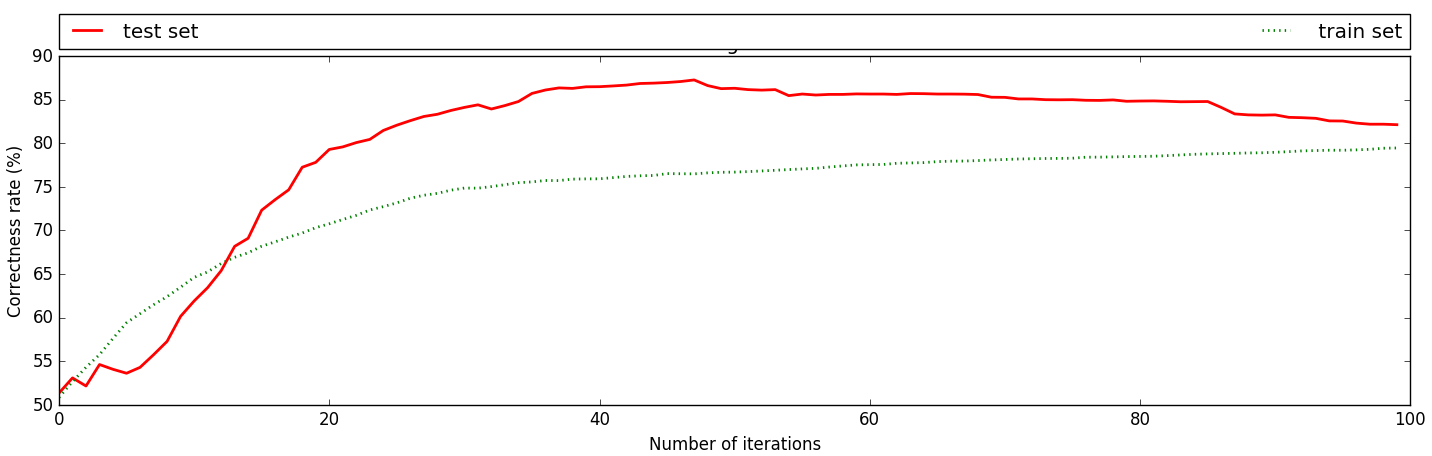
\includegraphics[width=.9\linewidth]{part7.png}
\caption{Learning curve}
\end{center}
\end{figure*}

With 67420 pairs of words in the training set, and 7108 pairs of words in the test set, the classifier correctly classified about 80 \% of the samples in both training and testing sets. \\

\end{homeworkProblem}


%----------------------------------------------------------------------------------------
%	PART 8
%----------------------------------------------------------------------------------------
\clearpage
\begin{homeworkProblem}
I used Ecludian distance to calculate the difference between the vectors. The two additional examples that I have are for the words \textit{best} and \textit{very}. \\

\textbf{10 words that are related to the word \textit{good} based on the embeddings are:} \\
perplexing
reinforcing
manipulate
wonderful
admiral
great
bad
funny
decent
underused \\

\textbf{10 words that are related to the word \textit{story} based on the embeddings are:} \\
ricci
film
acclaim
plot
domineering
benito
simmer
lift
interviews
sitter \\

\textbf{10 words that are related to the word \textit{very} based on the embeddings are:} \\
extremely
fairly
somewhat
pretty
skipping
too
sailboat
quite
oft
bit \\

\textbf{10 words that are related to the word \textit{best} based on the embeddings are:} \\
top
kyle
pounder
simplicity
popular
origins
worst
neal
morton
grahams \\
\end{homeworkProblem}




\end{document}